\section{Route Construction}
\label{sec:route}

\subsection{Saliency Field and Sparse Augmented Tree}

Let $I\in[0,1]^{H\times W\times3}$ be the normalized RGB image. A deterministic operator produces a saliency field $S\in[0,1]^{H_r\times W_r}$. The reference implementation uses frequency-tuned Lab contrast \cite{achanta2009frequency}, followed by Gaussian smoothing. The model reads RGB from $I$; $S$ is used only to build and describe the route.

A one-cell frame with a value below the range of $S$ closes contours that touch the image boundary. Each route-grid cell is split by the same northwest-to-southeast diagonal, and equal scalar values use a deterministic symbolic offset. We compute the full contour tree $T$ from this piecewise-linear field before selecting model routes. The padded rectangle is simply connected, so $T$ has no cycle. It may contain split and join saddles, but two siblings created by one split cannot later rejoin; a join combines branches with independent lower origins. A domain with holes would require a Reeb graph.

At $L$ retained regular levels, we extract closed contours, remove loops below simple perimeter and area thresholds, and insert the remaining loops on their tree arcs. Paths with no retained loop are contracted into a sparse execution tree $T_A$. The tree therefore fixes cross-level topology without forcing every fine branch to consume tokens. A normal-ray collision never creates or redirects a tree edge.

After smoothing $S$, we compute one $3\times3$ Sobel field $G=(G_x,G_y)$ on the route grid. All contours reuse this field.

\subsection{One Sobel Rule for Side, Density, and Anchor}

Let a retained contour $C$ have perimeter $P_C$ on the route grid. Its number of unique model points is fixed before adaptive placement:
\begin{equation}
N_C=\max\!\left(N_{\min},\operatorname{round}(P_C/\delta_0)\right).
\label{eq:budget}
\end{equation}
The default is $N_{\min}=16$ and $\delta_0=2$. There is no semantic upper cap: long loops use larger length buckets or exact chunked scans. Adaptive placement moves a fixed number of points; it never creates extra tokens for one region.

We orient $C$ clockwise and place $M_C=2N_C$ pilot points uniformly by arc length. Let $u_i$ be a pilot and $n_i$ its consistently oriented unit normal. Bilinear sampling of the Sobel field gives one signed normal response
\begin{equation}
r_i=G(u_i)^{\top}n_i.
\label{eq:sobel-response}
\end{equation}
Its sign says which normal side increases saliency. If the mean of $r_i$ is nonnegative, $+n_i$ is the high side and every ordinary ray uses $-n_i$; otherwise every ordinary ray uses $+n_i$. An exact zero uses the negative-normal side. This is one decision for the whole contour, not one decision per point.

The magnitude $g_i=|r_i|$ measures how quickly the saliency field changes across the contour. We smooth $g_i$ once around the loop with the circular kernel $(1,2,3,2,1)/9$, obtaining $\bar g_i$. Let $m_C$ be the median of the positive $\bar g_i$. If no positive response exists, all density weights are one. Otherwise,
\begin{equation}
w_i=\operatorname{clip}\!\left(\frac{\bar g_i}{m_C+\epsilon},1,3\right).
\label{eq:density}
\end{equation}
Thus weak regions keep the base density, strong changes receive more points, and the cap prevents a small region from consuming the loop budget. With uniformly spaced scalar levels, a larger normal derivative is also a first-order proxy for a smaller gap between neighboring level sets.

The anchor $p_0$ is the pilot with the largest smoothed, unclipped response $\bar g_i$. Ties use the lexicographically smallest image coordinate $(y,x)$. The same Sobel measurements therefore determine the read side, density, and start/end point without any pilot-stage collision query.

For a pilot interval of physical arc length $\Delta s_i$, assign mass
\begin{equation}
a_i=\Delta s_i\frac{w_i+w_{i+1}}{2}.
\end{equation}
Starting at $p_0$, we place exactly $N_C$ final points at equal increments of cumulative mass. The anchor is kept as the first point. High-weight intervals receive closer samples, but the count never changes. No sequence is stretched, truncated, or padded with invented geometry. Clockwise and counterclockwise scans use the same physical points in reverse order.

Only after redistribution do we cast geometric rays. A final point sends its ordinary ray on the selected loop-wide side until the first positive collision with a retained contour polyline or the padded frame. The starting contact and the two incident segments of $C$ are ignored. A terminal contour also casts the opposite-side ray. Route coordinates are mapped back to the original image, where RGB and saliency values are bilinearly sampled. Pilot points are never model tokens.

\begin{figure*}[t]
    \centering
    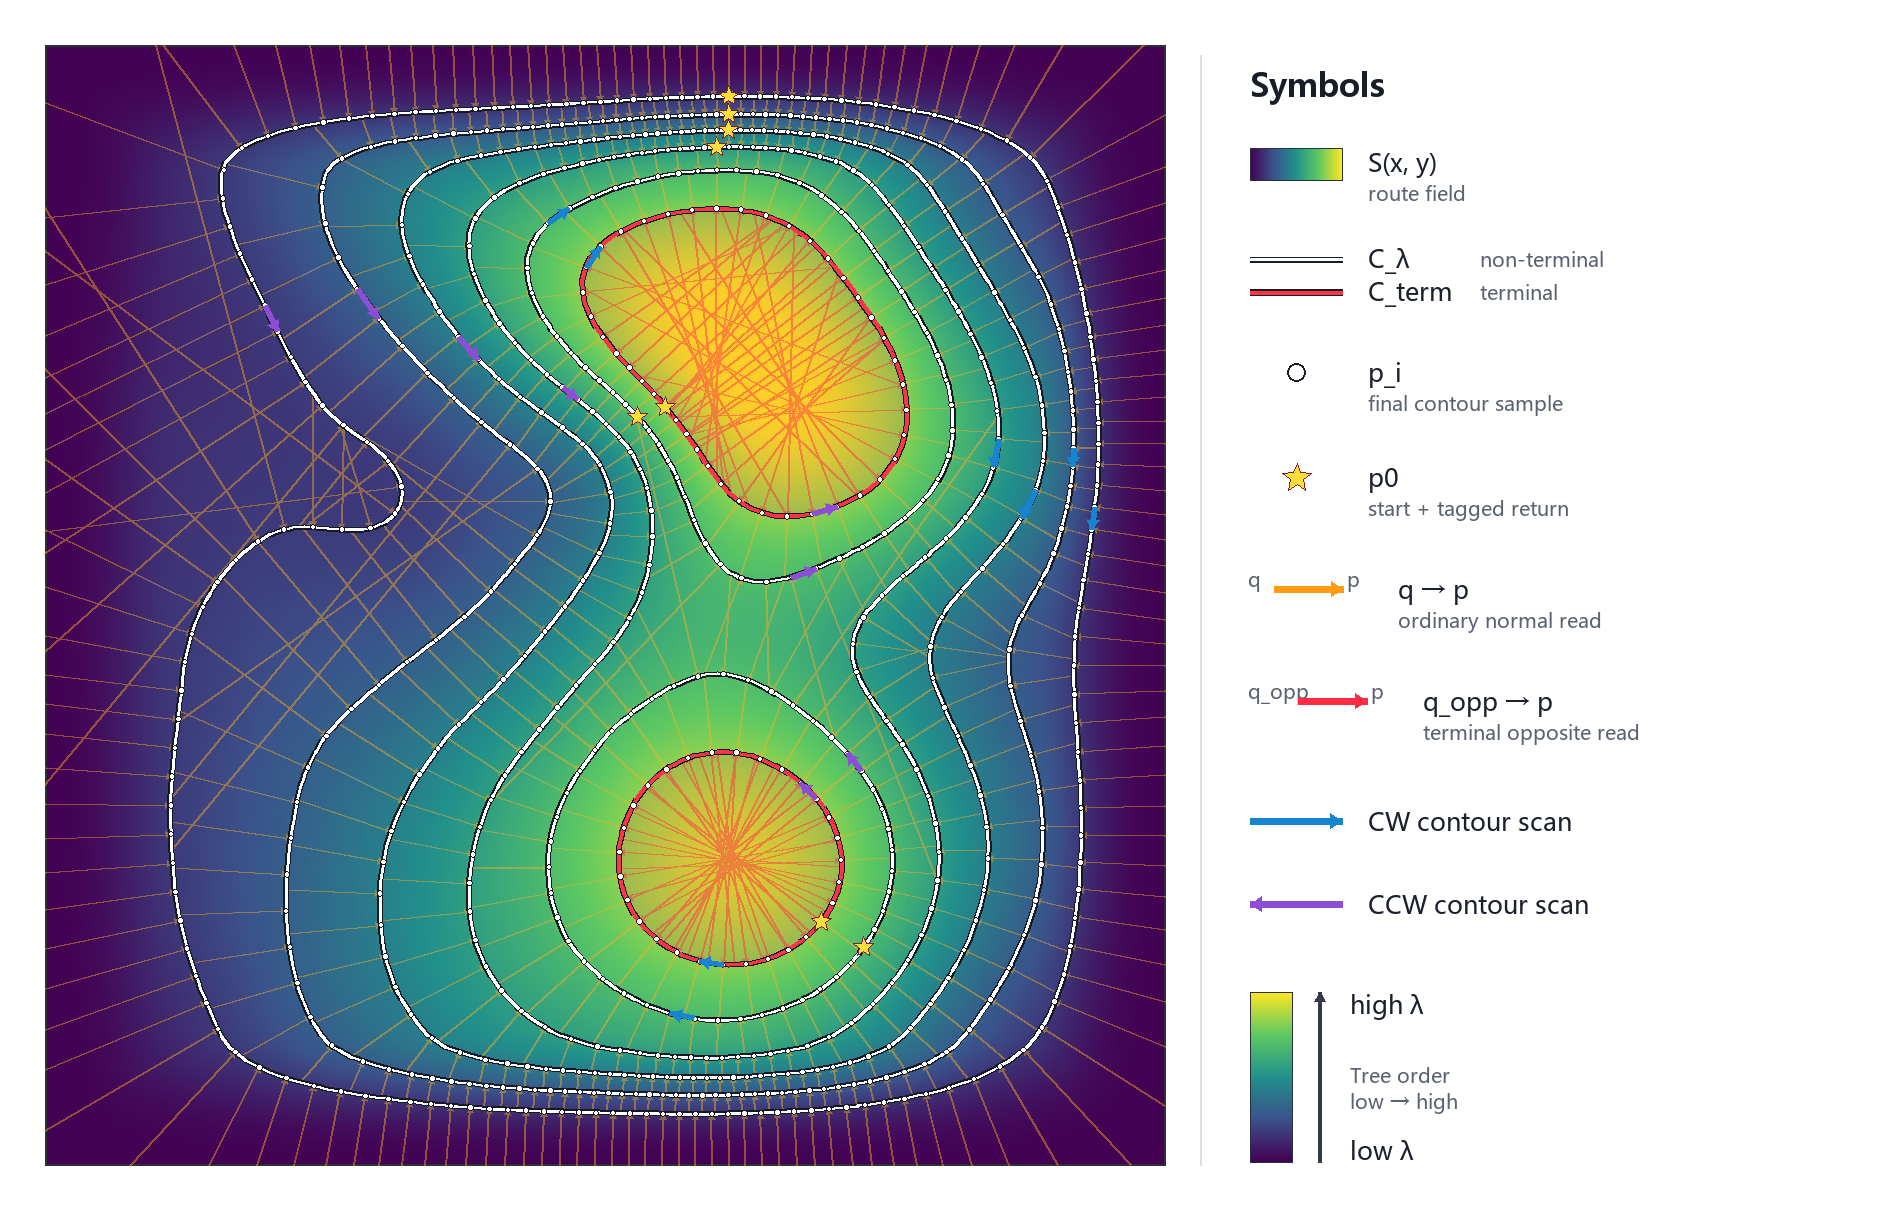
\includegraphics[width=0.84\textwidth]{figures/topocontour_paper_figure.png}
    \caption{One route generated by the specified rules. White curves are retained nonterminal contours; red curves and tinted interiors mark the last retained contour of each visible branch. Orange arrows show ordinary Normal Mamba reads from the first collision $q$ back to the contour point $p$; red arrows add the opposite-side reads used only at terminal contours. Stars mark the shared start and tagged return $p_0$, while blue and purple arrows show the two loop directions.}
    \label{fig:local}
    \vspace{0.35em}
    \begin{minipage}{0.84\textwidth}
    \small\textbf{Design philosophy.}
    The route does not declare low-saliency regions useless or remove them. It lets broad context enter the history early, with sparse placement where the Sobel field changes weakly, while sharper and terminal evidence is read later and remains closer to tagged outputs. Selective forgetting is therefore used as an attention schedule: weak context may fade but is still available, whereas distinctive evidence is less exposed to subsequent updates. This is an inductive bias rather than a memory guarantee. Because the geometry is fixed before scanning and every contour is locally independent, the image-specific order still permits parallel execution across rays and contours.
    \end{minipage}
\end{figure*}
